\documentclass{article}
\usepackage{amsmath} %For math equations
\usepackage{graphicx} % For images

\title{Practice}
\author{Md. Roman Nihal}
\date{March 2024}

\begin{document}

\maketitle

\section{Equations}

\begin{enumerate}
\item $(a+b)^2=a^2+2ab+b^2$
$(a-b)^2=a^2-2ab+b^2$
\item $(a-b)^2=a^2-2ab+b^2$
$$(\frac{4}{2}+5)^2=49$$
$$\left(\frac{4}{2}+5\right)^2=49$$
$$(a+b)^{2+\pi}$$
$$\alpha=\beta=\gamma=\Gamma=\lambda=\Lambda=\pi=\Pi=\epsilon$$
\end{enumerate}

\begin{itemize}
\item $x^2+\frac{25x^2}{(x+5)^2}=11$
\item $T`=T\sqrt{1-\frac{v^2}{c^2}}$
$$F_G=\frac{GM_1M_2}{r^2}$$
$$limit_{n\to\infty}=\frac{n}{\sqrt[n]{n!}}$$
$$e=\sum^{\infty}_{n=0}\frac{1}{n!}$$
$$e=2+\frac{1}{1+\frac{1}{2+\frac{2}{3+\ddots}}}$$
\end{itemize}

\section{More}

$$\int_a^bf(x)dx$$
$$\iiint f(x,y,z)dxdydz$$
$$\Vec{v}=<v_1 v_2 v_3>$$
$$\Vec{v}\cdot\Vec{w}$$

$$\begin{bmatrix}
    1&2&3\\
    4&5&6\\
    7&8&9
\end{bmatrix}$$

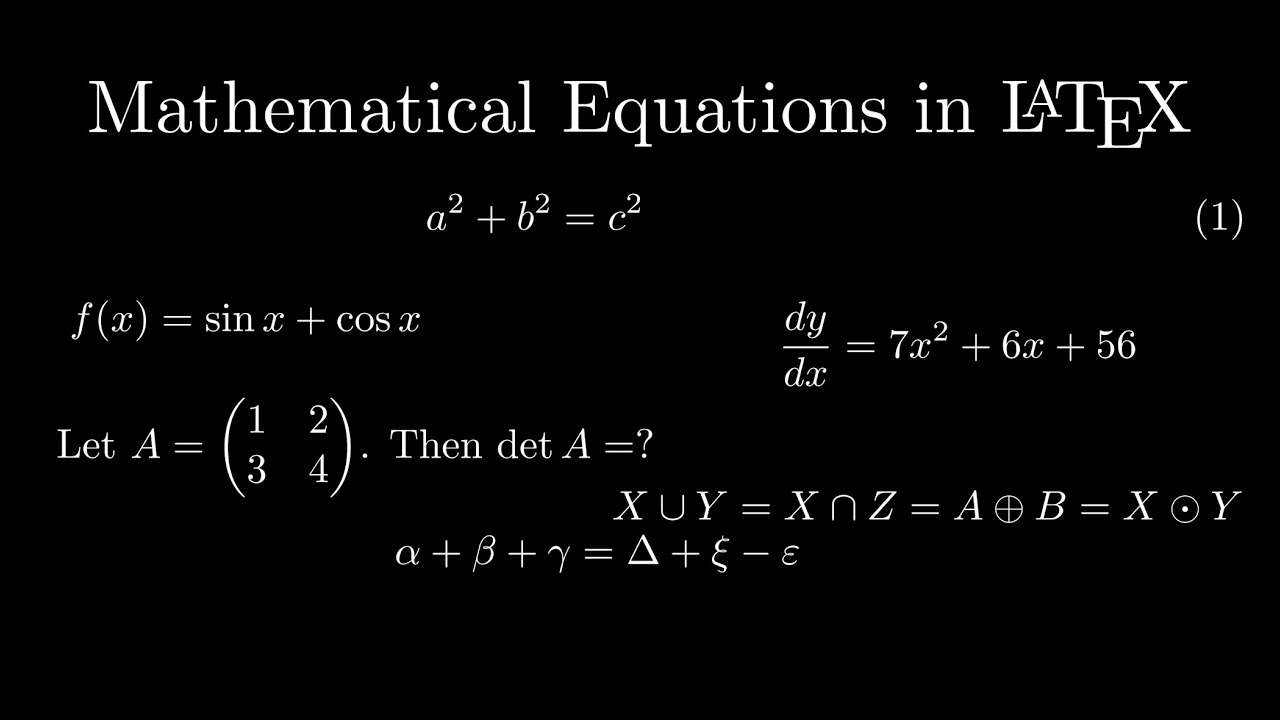
\includegraphics[scale=0.25]{eq.jpg}\centering
\end{document}
